%=========================================================================
\chapter{The RdRand instruction}  \label{chap:rdrand-instruction}
First public information about RdRand came somewhen during year 2011\cite{IntelRdRandFindAbout}, a~year before the~CPUs with it were released and Intel itself send patches to add support into Linux in summer of~the~same year\cite{KernelRdRand}. Later, RdRand was added between Linux entropy sources for {\tt /dev/[u]random}.\TODO{Find discussion}% TODO find discussion
According to known information\cite{TheodoreTsoNSA}, Intel tried to have {\tt /dev/[u]random} rely only on their instruction, but that was denied. 

We weren't able to find any relevant data about usage of~RdRand in Windows kernel, probably because all such negotiations happened behind closed doors. In user space, there is no difference between Linux and Windows; when it is possible to call the~instruction, user space applications can use it. 

After disclosure of~extends of~NSA spying activities by Edward Snowden in summer of~2013\cite{GuardianNSA}\cite{DailymailNSA}, a~petition for removing RdRand from Linux entropy sources was created\cite{PetitionRdRand}. Although supported by just 8 signatures, it got wide attention on information-technology aimed news pages and magazines, like Slashdot.org\cite{PetitionRdRandSlashdot}. The petition was closed after Linus Torvalds responds with scorn:

\begin{quote} ...

Short answer: we actually know what we are doing. You don't.

Long answer: we use rdrand as \_one\_ of~many inputs into the~random pool, and we use it as a~way to \_improve\_ that random pool. So even if rdrand were to be back-doored by the~NSA, our use of~rdrand actually improves the~quality of~the~random numbers you get from {\tt /dev/random}.

...
\end{quote}


% --------------------------------------------------------
\section{Intel Secure Key}\label{sec:intel-secure-key}
The Intel Secure Key (ISK) uses cascade construction, combining a~HW RNG with CSPRNG into one sealed block on CPU, which is compliant with many security standards, including NIST SP800-90, FIPS-140-2, and ANSI X9.82\cite{IntelDRNGGuide}. Although it is impossible to audit it, there was found no evidence of~low entropy or anything that would deny the~security standards compliance - neither with tests in \fullref{chap:statistical-testing}, nor any other tests anyone else did\footnote{I assume that such revelation would become quickly known and broadly discussed.}.

% --------------------------------------------------------
\section{Physical implementation}\label{sec:ISK-physical}
One important thing about ISK, that has big impact on performance, but also price of~that solution is, that there is only one unit on a~die and the~unit should be the~same on all CPUs.\TODO{quote it} % TODO quote it
Because all processing units (PU)\footnote{Two physical cores with hyper-threading counts as four PU.} on one die share the~RNG, one thread reading random numbers from it can never be faster than $Total speed  \frac{1}{PUs}$. The effect of~this is that the~performance is perfectly scalable (see \fullref{chap:performance}), and price of~the~CPU is less affected.

Each ISK unit consists three basic parts: A hardware entropy source, a~conditioner and a~{\em deterministic random bit generator} (DRBG)\cite{IntelDRNGGuide}. The frequency of~the~RNG is independent on the~rest of~the~CPU and is set to 800 MHz. 
\begin{figure}[h!]
  \centering
 \includegraphics[width = 10cm,keepaspectratio]{fig/ISK-scheme.pdf} % Or .pdf
%\includegraphics[width=10cm,keepaspectratio]{fig/ISK-scheme}
\caption{An Intel Secure Key unit}
\label{fig:ISK-unit}
\end{figure}


% ....................................................
\subsection{Entropy source}

The entropy source is a~metastable circuit, with unpredictable behavior based 
on thermal noise\cite{UnderstandingRdRandElectronic}. 
In figure~\ref{fig:ES-circuit}, the~middle (red) part is the~heart 
of~the~circuit, a~RS-NOR latch. As its {\em reset} and {\em set} inputs 
are wired together, when an impulse is brought on these inputs, the~latch sets 
to 1 or 0 based on thermal noise. To provide better distribution, there is 
the~bottom (blue) negative feedback. Based on the~output of~the~latch, charge 
on capacitors in the~negative feedback is adjusted and then this negative 
feedback slightly shift the~chance for next bit to be opposite. The longer 
is a~sequence of~the~same bits, the~higher charge is on the~capacitors 
and bigger effect it has.

Finally, when the~latch is settled in one state, the~top (green) part 
of~the~circuit detect it, saves the~bit (and send it further), wait 
a~little time and then it sends a~pulse on the~R/S inputs of~the~latch 
to produce a~new bit. This entropy source has its own frequency, different 
from the~rest of~the~RNG, about 3~GHz.

\begin{figure}[h!]
  \centering
 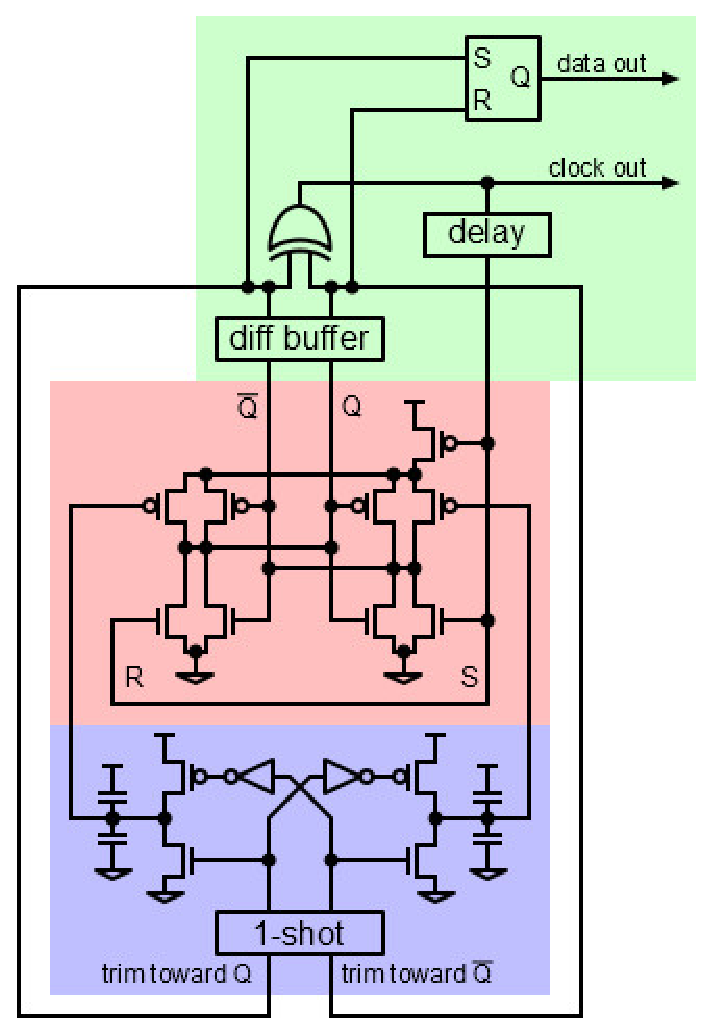
\includegraphics[width=6cm,keepaspectratio]{fig/entropy-source-circuit} % Or .pdf
%\includegraphics[width=10cm,keepaspectratio]{fig/ISK-scheme}
\caption{Circuit scheme of~the~entropy source\cite{UnderstandingRdRandElectronic}.}
\label{fig:ES-circuit}
\end{figure}

% ....................................................
\subsection{Conditioner}
The entropy source provides random bits with some entropy, but due to implementation and the~feedback, it can be unbalanced and produce values in something close to oscillating patterns. For this reason, there is the~conditioner that adds them to a~256 bit pool, make a~set of~XOR and AES operations over lower and upper half of~the~pool and test health of~the~pool\footnote{The health check is done by counting six different bit patterns in the~256 bit pool and comparing the~counts with empirically chosen values. The pool is healthy only if the~numbers are in the~specified ranges.}\cite{AnalysisOfDRNG}\cite{UnderstandingRdRandElectronic}. If the~pool is not healthy, the~set of~operations is repeated. 

% ....................................................
\subsection{DRBG}\label{subsec:DRBG}
Because the~output speed of~the~conditioner is too slow (just 256 bits per few microseconds), a~deterministic random bit generator is connected to the~256 bit pool and every few microseconds (if the~pool is healthy) takes it as a~new seed. This pseudo random generator then compute 65.536 bits values using an 128-bit AES and put them to a~output buffer. From there, they can be taken by the~RdRand instruction after 64-bit blocks\footnote{64 bits are always taken out, no matter what size is the~target register of~the~instruction. Thus, it is not possible to achieve the full speed of the DRBG on 32-bit system, as there is no difference for the Intel Secure Key usage, just some bits are later thrown away. See \fullref{subsec:32vs64} for a performance test.}\cite{AnalysisOfDRNG}\cite{UnderstandingRdRandElectronic}. Reseeding of~the~DRBG is required after all 1024 blocks are used, but usually it will reseed more frequently.

% ....................................................
\subsection{Built-in self-tests (BIST)}
Intel Secure Key contain also built-in self tests. After a reset, the BIST at first test health of the DRBG and conditioner, then it test the entropy source. In the first part, ES is disconnected, a previously determined bit sequence is 'generated' and the BIST checks the output with a built-in value. In second phase, the entropy source is connected and few sequences are generated. If the entropy source would be bad, the previously checked health check in conditioner would detect it. 

In case one of the BIST parts would not be finished correctly and the RdRand instruction is called, just zeros are returned and carry flag is cleared\cite{AnalysisOfDRNG}.

% --------------------------------------------------------
\section{Existing usages} 
Some well known projects that already have support for RdRand are the Linux kernel, OpenSSL, ...
\TODO{write more}% TODO write more


%========================================================================= 
